\documentclass{article}

\usepackage[margin=3cm]{geometry}

\usepackage{fancyhdr}
\pagestyle{fancy}
\usepackage{graphicx}
\usepackage{color}
\usepackage{xcolor}
\definecolor{code}{rgb}{.92,.92,.99}
\definecolor{codered}{rgb}{.92,.62,.62}
\definecolor{darkgreen}{rgb}{.2,.62,.18}
\usepackage{listings}
\lstset{xrightmargin=10pt,xleftmargin=10pt,language=Java,captionpos=b,tabsize=3,frame=none,keywordstyle=\color{blue},commentstyle=\color{darkgreen},stringstyle=\color{red},showstringspaces=false,basicstyle=\footnotesize\ttfamily,emph={label},backgroundcolor=\color{code}}
%%numbers=left,numberstyle=\tiny,numbersep=5pt,breaklines=true,\

\newenvironment{code}
{\begin{minipage}[l]{\textwidth}}
{\end{minipage}}

\newcommand{\ccpmaketitle}[3] {
	\fancyhead[LO,LE]{Crash Course Paparazzi 2016}
	\fancyfoot[LO,LE]{{\small introPaparazzi}}
	\fancyfoot[CO,CE]{\thepage}
	\author{Roland Meertens, Christophe de Wagter, Guido de Croon}
	\title{\bf Crash Course Paparazzi 2016\\#1\\{\large #3#2}}
	\date{Februari 2016}
	\setlength{\parindent}{0em}
	\maketitle
}

\usepackage{graphicx}

\begin{document}
\ccpmaketitle{Computer vision}{\ldots Making your drone see something}{lesson 4}

\subsection*{Introduction}
Welcome to the most important part of this course: understanding how vision works. When using image processing right your drone can perform the most awesome tricks. However: when you do it wrong your drone will fall to the ground. 

\subsection*{Goals of this exercise}
\begin{itemize}
\item Finding the camera data
\item The format of the image
\item Your first project
\end{itemize}

\subsection*{Finding the camera data}
To get data out of the camera in paparazzi you have to include the video\_thread.xml module in your airframe file, and define VIDEO\_THREAD\_CAMERA to front\_camera. Your modules section now looks like this:
\begin{verbatim}
<modules>
XXXXX
</modules>
\end{verbatim}
After you added this you can create a new module that does something with the data of the front camera. A nice example for such a module is the colorfilter module. Take some time to check what the colorfilter does in the file colorfilter.c. 

In the colorfilter\_init function the function cv\_add is called with as argument the colorfilter\_func function:
\begin{verbatim}
Code here
\end{verbatim}
Now each time the video thread gets an image from the camera it calls the colorfilter\_func function with the new image as an argument:
\begin{verbatim}
Code here
\end{verbatim}
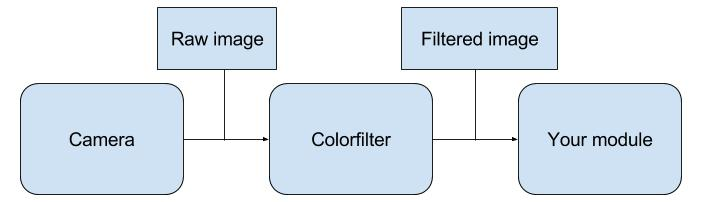
\includegraphics[width=0.8\linewidth]{camerafilter}

Note that the order in which you call cv\_add is important. The first function to get the image might edit the image. If you add modules that do something with the image, the first module you added in your flightplan will get the image first. The reason that the image might be changed can be found in the way the image is given to a function: 
\begin{verbatim}
Code on how the image is called hee
\end{verbatim}
As the argument the function gets is a pointer to an image it is possible for a module to change the actual image. If you take a look at the colorfilter function you soo this module does this. By adding a colorfilter that filters on orange, a second module added after the colorfilter will only see orange. 

\subsection*{The format of the image}
Currently I don't know what format is used. Too bad...

\subsection*{Your first project}
Now it is time to choose an exercise to learn how to program in Paparazzi using your flightplan skills, code skills and computer vision skills. The two options are:

\subsubsection*{Choice 1: Read a sign}
Fly to a position in the center of the arena. If you see a blue sign fly to a waypoint to the left, hover here for five seconds and go back to the center. If you see a red sign perform the same behaviour but fly to the right. 

\subsubsection*{Choice 2: Follow me!}
Create a real "selfie-drone" in which the drone follows an orange blob at a certain distance. 
Start by hovering at a waypoint and determining where the orange blob is (more to the left or more to the right?) and adjust your heading based on this. 
To start following you you can determine the size of the blob. Is it too big? Fall back! Otherwise: fly forwards by replacing your waypoint.
\end{document}
